\section{Mạng Sinh đối nghịch (Generative Adversarial Networks - GANs)}
\label{sec:gans}

Trước năm 2014, để máy tính sinh ra một bức ảnh mới, các nhà nghiên cứu phải xây dựng các mô hình xác suất phức tạp, ước lượng trực tiếp phân phối dữ liệu --- một bài toán cực kỳ khó trong không gian hàng triệu chiều (số pixel của ảnh). Năm 2014, Ian Goodfellow đề xuất \textbf{Generative Adversarial Networks (GAN)} \cite{Goodfellow2014} với một ý tưởng hoàn toàn khác: thay vì ước lượng phân phối, hãy để \textit{hai mạng nơ-ron tự dạy nhau}.

\subsection{Ý tưởng Cốt lõi: Trò chơi Tiền giả và Cảnh sát}
\label{subsec:gan_core_idea}

Hãy tưởng tượng một kẻ làm tiền giả (Generator) và một cảnh sát (Discriminator). Ban đầu, kẻ làm giả không biết gì về tiền thật, in ra những tờ tiền trông rất buồn cười. Cảnh sát dễ dàng phát hiện. Kẻ làm giả quan sát phản ứng của cảnh sát và cải thiện kỹ thuật. Cảnh sát giỏi hơn buộc kẻ làm giả phải giỏi hơn. Vòng lặp này cứ tiếp diễn cho đến khi tờ tiền giả trông hệt như thật.

GAN hiện thực hóa câu chuyện đó với hai mạng nơ-ron:

\begin{center}
	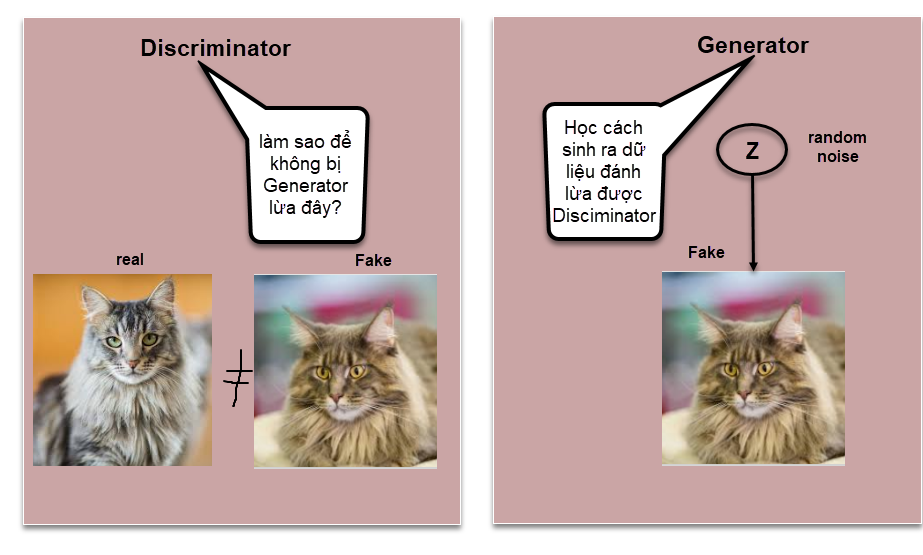
\includegraphics[width=0.95\textwidth]{images/gan_overview.png}
	\captionof{figure}{Kiến trúc tổng quan GAN: Generator nhận noise $\mathbf{z}$ và sinh ảnh giả; Discriminator nhận cả ảnh thật lẫn ảnh giả và phân loại; tín hiệu lỗi từ Discriminator được dùng để cập nhật Generator.}
	\label{fig:gan_overview}
\end{center}

\textbf{Generator (G) --- Từ nhiễu ngẫu nhiên đến ảnh.}
Đây là câu hỏi trọng tâm: \textit{Generator sinh ảnh ra kiểu gì?}

Generator là một mạng nơ-ron nhận đầu vào là một \textbf{vector nhiễu ngẫu nhiên} $\mathbf{z} \in \mathbb{R}^d$ (thường $d = 100$), lấy mẫu từ phân phối đơn giản như Gaussian $\mathcal{N}(0, I)$, và biến đổi nó thành một ảnh $G(\mathbf{z}) \in \mathbb{R}^{H \times W \times 3}$. Về bản chất, Generator học một \textbf{hàm ánh xạ} từ không gian nhiễu sang không gian ảnh:

\[
G: \mathbb{R}^d \rightarrow \mathbb{R}^{H \times W \times C}, \quad \mathbf{z} \mapsto \hat{\mathbf{x}}
\]

Kiến trúc của Generator --- ở dạng đơn giản nhất (GAN gốc) --- là một MLP nhiều lớp với BatchNorm và ReLU:

\begin{center}
	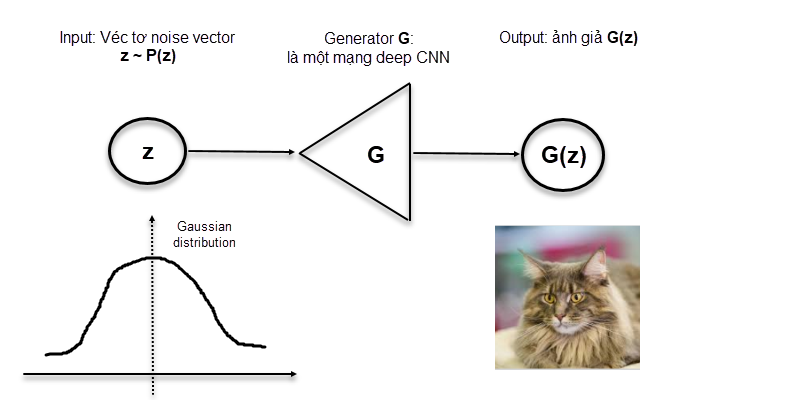
\includegraphics[width=0.90\textwidth]{images/gan_generator_arch.png}
	\captionof{figure}{Kiến trúc Generator: vector noise $\mathbf{z}$ (100 chiều) đi qua các lớp Linear → BatchNorm → ReLU, cuối cùng Tanh để ra ảnh có giá trị pixel trong $[-1, 1]$.}
	\label{fig:gan_generator}
\end{center}

Cụ thể với ảnh $28\times28$ (MNIST), luồng biến đổi là:
\[
\mathbf{z} \in \mathbb{R}^{100} \xrightarrow{\text{Linear+BN+ReLU}} \mathbb{R}^{256} \xrightarrow{\text{Linear+BN+ReLU}} \mathbb{R}^{512} \xrightarrow{\text{Linear+BN+ReLU}} \mathbb{R}^{1024} \xrightarrow{\text{Linear+Tanh}} \mathbb{R}^{784}
\]
Vector 784 chiều được reshape thành ảnh $28 \times 28$. Mỗi giá trị $z_i$ trong vector noise điều khiển một \textit{khía cạnh tiềm ẩn} của ảnh được sinh ra (tư thế, kiểu tóc, ánh sáng...) --- dù G không được dạy tường minh điều đó, nó tự học trong quá trình training.

\textbf{Discriminator (D) --- Thám tử phân loại thật/giả.}
Discriminator là một bộ phân loại nhị phân: nhận vào một ảnh $\mathbf{x}$ và xuất ra xác suất $D(\mathbf{x}) \in [0,1]$ thể hiện khả năng ảnh đó là \textit{thật}.

\begin{center}
	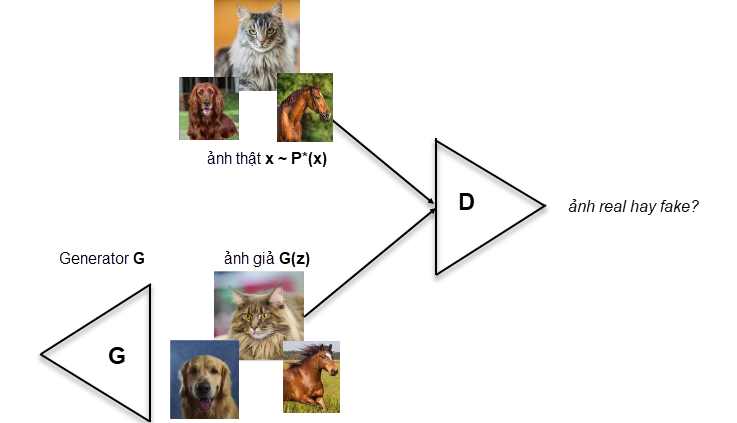
\includegraphics[width=0.90\textwidth]{images/gan_discriminator_arch.png}
	\captionof{figure}{Kiến trúc Discriminator: ảnh đầu vào (thật hoặc giả) đi qua các lớp Linear → LeakyReLU, cuối cùng Sigmoid để xuất ra xác suất $D(\mathbf{x}) \in [0,1]$.}
	\label{fig:gan_discriminator}
\end{center}

D dùng LeakyReLU thay vì ReLU để tránh dead neuron --- đây là chi tiết kỹ thuật quan trọng vì D cần gradient mạnh để học phân biệt tốt. Với ảnh thật: $D(\mathbf{x}) \rightarrow 1$; với ảnh giả: $D(G(\mathbf{z})) \rightarrow 0$.

\textbf{Hàm mất mát Minimax --- Hai mạng tối ưu ngược chiều nhau.}
Trò chơi đối kháng được hình thức hóa bằng một hàm mục tiêu duy nhất:
\begin{equation}
	\min_{G}\, \max_{D}\; V(D,G) = \underbrace{\mathbb{E}_{\mathbf{x} \sim p_{\text{data}}}[\log D(\mathbf{x})]}_{\text{D phân loại đúng ảnh thật}} + \underbrace{\mathbb{E}_{\mathbf{z} \sim p_{\mathbf{z}}}[\log(1 - D(G(\mathbf{z})))]}_{\text{D phân loại đúng ảnh giả}}
\end{equation}

\begin{itemize}
	\item \textbf{D muốn tối đa hóa} $V$: đưa $D(\mathbf{x}_\text{real}) \to 1$ (nhận đúng ảnh thật) và $D(G(\mathbf{z})) \to 0$ (nhận đúng ảnh giả).
	\item \textbf{G muốn tối thiểu hóa} $V$: làm $D(G(\mathbf{z})) \to 1$ để $\log(1 - D(G(\mathbf{z}))) \to -\infty$, tức là đánh lừa D tin ảnh giả là thật.
\end{itemize}

Hai mạng kéo nhau theo hai hướng ngược --- đó là bản chất của adversarial training.

\textbf{Vòng lặp huấn luyện xen kẽ.}
Vì G và D cạnh tranh nhau, chúng không thể tối ưu đồng thời. GAN dùng chiến lược \textbf{huấn luyện xen kẽ} --- mỗi iteration gồm hai bước:

\begin{enumerate}
	\item \textbf{Bước 1 --- Cập nhật D (giữ G cố định):}
	\begin{itemize}
		\item Lấy batch ảnh thật $\{\mathbf{x}^{(i)}\}$ từ dataset.
		\item Sinh batch ảnh giả $\{G(\mathbf{z}^{(i)})\}$ với noise lấy mẫu mới.
		\item Tính loss của D: $\mathcal{L}_D = -\frac{1}{m}\sum_i \left[\log D(\mathbf{x}^{(i)}) + \log(1 - D(G(\mathbf{z}^{(i)})))\right]$
		\item Gradient ascent để cực đại hóa (hay tương đương, gradient descent với $-\mathcal{L}_D$).
		\item Cập nhật \textit{chỉ} trọng số của D.
	\end{itemize}

	\item \textbf{Bước 2 --- Cập nhật G (giữ D cố định):}
	\begin{itemize}
		\item Sinh batch noise mới $\{\mathbf{z}^{(i)}\}$, tạo ảnh giả $\{G(\mathbf{z}^{(i)})\}$.
		\item Tính loss của G: $\mathcal{L}_G = -\frac{1}{m}\sum_i \log D(G(\mathbf{z}^{(i)}))$
		\item Gradient descent cực tiểu hóa $\mathcal{L}_G$ --- tức là tối đa hóa xác suất D bị đánh lừa.
		\item Cập nhật \textit{chỉ} trọng số của G.
	\end{itemize}
\end{enumerate}

Lưu ý: trong bước 2, G dùng loss $-\log D(G(\mathbf{z}))$ thay vì $\log(1-D(G(\mathbf{z})))$ trong công thức gốc --- đây là \textbf{Non-Saturating GAN loss}. Lý do: khi G yếu (đầu training), $D(G(\mathbf{z})) \approx 0$, gradient của $\log(1-D)$ tiến về 0 (vanishing gradient), còn gradient của $-\log D$ vẫn lớn, giúp G học nhanh hơn.

\textbf{Điểm cân bằng Nash --- Khi nào GAN hội tụ?}
Lý thuyết chứng minh rằng trạng thái cân bằng lý tưởng đạt được khi $p_G = p_{\text{data}}$ (phân phối ảnh giả bằng phân phối ảnh thật), và tại đó D không còn phân biệt được nữa --- nó chỉ đoán ngẫu nhiên $D(\mathbf{x}) = 0.5$ với mọi $\mathbf{x}$. Tuy nhiên, trong thực tế, hội tụ về Nash equilibrium là \textit{không được đảm bảo} và quá trình training GAN nổi tiếng là bất ổn.

\begin{mdframed}[style=infobox]
\textbf{Hai vấn đề cổ điển khi huấn luyện GAN}

\textbf{1. Vanishing Gradient (Gradient biến mất):}
Nếu D quá giỏi so với G --- tình huống thường xảy ra đầu training --- D phân loại ảnh giả gần như hoàn hảo: $D(G(\mathbf{z})) \approx 0$. Khi đó $\log(1 - D(G(\mathbf{z}))) \approx \log(1) = 0$, gradient truyền về G gần bằng 0. G không nhận được tín hiệu để cải thiện --- training bị kẹt.

\textbf{2. Mode Collapse (Sụp đổ mode):}
G khám phá ra một ``đường tắt'': thay vì học phân phối đa dạng của dữ liệu thật, nó chỉ sinh ra \textit{một vài dạng ảnh} trông đủ thật để đánh lừa D. Ví dụ, khi huấn luyện trên MNIST, G chỉ sinh ra số 8 (vì 8 trông đủ tròn để D nhầm là thật) và bỏ qua các chữ số còn lại. D thích nghi để nhận ra điều này, nhưng G lại chuyển sang một mode khác, rồi G lại chuyển... Hai mạng đuổi nhau vòng vòng mà không hội tụ.

Cả hai vấn đề này là động lực để WGAN ra đời với khoảng cách Wasserstein --- sẽ được trình bày ngay sau đây.
\end{mdframed}

\begin{center}
	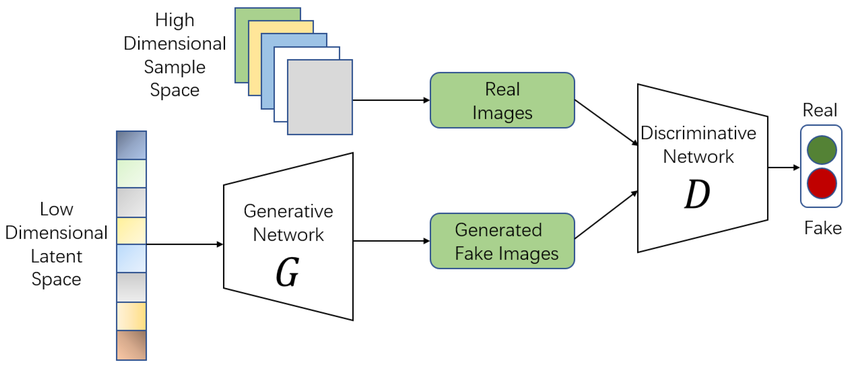
\includegraphics[width=0.9\textwidth]{images/gan_architecture_diagram.png}
	\captionof{figure}{Luồng gradient trong GAN: tín hiệu loss từ D lan truyền ngược qua G để cập nhật trọng số của Generator. D được cập nhật riêng với cả ảnh thật và ảnh giả.}
	\label{fig:gan_architecture}
\end{center}

\subsection{Các Kiến trúc Nền tảng: DCGAN và WGAN}
\label{subsec:dcgan_wgan}

Các GAN gốc sử dụng mạng fully-connected, dẫn đến khó khăn trong việc học các cấu trúc phức tạp của ảnh và chỉ tạo ra hình ảnh chất lượng thấp. Để khắc phục, hai kiến trúc nền tảng là \textbf{DCGAN} và \textbf{WGAN} ra đời, mỗi kiến trúc giải quyết một khía cạnh quan trọng: khả năng học biểu diễn hình ảnh và ổn định huấn luyện.

\subsubsection{DCGAN (2015): Tích hợp Tích chập}
\label{subsubsec:dcgan}

\textbf{Deep Convolutional GAN (DCGAN)} \cite{Radford2015} là bước đột phá cho GAN trên ảnh. DCGAN đề xuất một tập các nguyên tắc thiết kế giúp huấn luyện ổn định và tạo ra ảnh chất lượng cao:

\begin{itemize}
	\item \textbf{Thay lớp pooling bằng convolution:}  
	\begin{itemize}
		\item Trong Discriminator: sử dụng \textbf{strided convolution} để giảm chiều ảnh (downsampling).  
		\item Trong Generator: sử dụng \textbf{transposed convolution} (tích chập chuyển vị) để tăng chiều ảnh (upsampling).
	\end{itemize}
	\item \textbf{Batch Normalization:} Ổn định gradient, giúp quá trình huấn luyện mượt mà hơn cho cả Generator và Discriminator.
	\item \textbf{Loại bỏ fully-connected layers sâu:} Giảm sự phụ thuộc vào các kết nối toàn phần, tập trung học các đặc trưng không gian.
	\item \textbf{Chức năng kích hoạt:} ReLU cho Generator (ngoại trừ lớp đầu ra dùng Tanh), LeakyReLU cho Discriminator.
\end{itemize}

\textbf{Kết quả:}  
DCGAN tạo ra các ảnh có độ phân giải cao hơn, chân thực hơn (ví dụ: phòng ngủ, khuôn mặt). Nó cũng chứng minh rằng \textbf{không gian tiềm ẩn (latent space) học được các biểu diễn có ý nghĩa} – ví dụ, phép cộng vector trong latent space có thể mô phỏng các thay đổi ngữ nghĩa:  
\[
\text{“người đàn ông đeo kính”} - \text{“người đàn ông”} + \text{“người phụ nữ”} \approx \text{“người phụ nữ đeo kính”}.
\]

\subsubsection{WGAN (2017): Giải quyết Vấn đề Ổn định và Mode Collapse}
\label{subsubsec:wgan}

Một vấn đề lớn của GAN truyền thống là \textbf{mode collapse}, khi Generator chỉ học tạo ra một vài mẫu ảnh giả cực tốt, bỏ qua phần còn lại của phân phối dữ liệu thật. Đồng thời, quá trình huấn luyện thường không ổn định.

\textbf{Wasserstein GAN (WGAN)} \cite{Arjovsky2017} cải thiện GAN bằng hai ý tưởng chính:

\begin{itemize}
	\item \textbf{Khoảng cách Wasserstein-1:}  
	Thay vì đo lường sự khác biệt giữa hai phân phối bằng Jensen-Shannon divergence, WGAN dùng \textbf{Earth-Mover (EM) distance} để đo khoảng cách giữa phân phối thật và phân phối giả. EM distance mượt mà, cung cấp gradient có ý nghĩa ngay cả khi hai phân phối không chồng lên nhau.
	
	\item \textbf{Hàm mất mát WGAN:}
	\begin{align}
		\mathcal{L}_D &= \mathbb{E}_{\mathbf{x} \sim p_{\text{data}}} [D(\mathbf{x})] - \mathbb{E}_{\tilde{\mathbf{x}} \sim p_g} [D(\tilde{\mathbf{x}})] \\
		\mathcal{L}_G &= \mathbb{E}_{\tilde{\mathbf{x}} \sim p_g} [D(\tilde{\mathbf{x}})]
	\end{align}
	
	\item \textbf{Điều kiện Lipschitz:}  
	Critic (Discriminator trong WGAN) cần thỏa mãn điều kiện 1-Lipschitz để hàm mất mát có ý nghĩa. WGAN ban đầu dùng \textbf{weight clipping}, nhưng WGAN-GP (Gradient Penalty) cải tiến bằng cách thêm một thành phần phạt gradient, đảm bảo norm của gradient bằng 1.
\end{itemize}

\textbf{Hiệu quả:}  
WGAN và WGAN-GP giúp huấn luyện GAN ổn định hơn, giảm đáng kể mode collapse và cung cấp gradient tốt cho Generator ngay cả khi phân phối dữ liệu thật và giả gần như không chồng lấn.

\subsection{StyleGAN: Làm chủ Phong cách và Chi tiết}
\label{subsec:stylegan}

\textbf{StyleGAN} \cite{Karras2019}, được NVIDIA giới thiệu vào năm 2018, đã tạo ra một cuộc cách mạng trong việc sinh ảnh chân thực với khả năng điều khiển chi tiết từng phần của hình ảnh. Các phiên bản kế nhiệm \textbf{StyleGAN2} và \textbf{StyleGAN3} tiếp tục nâng cao chất lượng, loại bỏ artifact và cải thiện tính bất biến cho video và hình động.

\subsubsection{Kiến trúc Generator dựa trên phong cách (Style-based Generator)}

Khác với GAN truyền thống, StyleGAN tách biệt \textbf{không gian tiềm ẩn} và \textbf{quá trình sinh ảnh}, cho phép kiểm soát các thuộc tính ảnh ở nhiều cấp độ.

\begin{enumerate}
	\item \textbf{Mapping Network:} 
	\begin{itemize}
		\item Vector tiềm ẩn $\mathbf{z}$ được lấy từ phân phối chuẩn (Gaussian) không được đưa trực tiếp vào Generator.
		\item Thay vào đó, $\mathbf{z}$ được đưa qua một MLP gọi là \textbf{Mapping Network} để tạo ra vector trung gian $\mathbf{w}$ nằm trong không gian “ít vướng víu” (less entangled). 
		\item $\mathbf{w}$ là vector điều khiển các đặc trưng hình ảnh mà Generator sinh ra, giúp kiểm soát các phong cách một cách trực quan.
	\end{itemize}
	
	\item \textbf{Adaptive Instance Normalization (AdaIN):} 
	\begin{itemize}
		\item $\mathbf{w}$ được ánh xạ thành các tham số \textbf{scale} và \textbf{bias} dùng trong module AdaIN để điều khiển output của từng lớp tích chập.
		\item Công thức AdaIN:
		\begin{equation}
			\text{AdaIN}(\mathbf{x}_i, \mathbf{y}) = \mathbf{y}_{s,i} \frac{\mathbf{x}_i - \mu(\mathbf{x}_i)}{\sigma(\mathbf{x}_i)} + \mathbf{y}_{b,i}
		\end{equation}
		Trong đó, $\mathbf{x}_i$ là feature map tại lớp i, và $\mathbf{y}_{s,i}, \mathbf{y}_{b,i}$ là scale và bias được sinh từ $\mathbf{w}$.
		\item AdaIN giúp điều khiển các thuộc tính khác nhau ở từng lớp: 
		\begin{itemize}
			\item Lớp đầu: điều khiển các đặc trưng thô như tư thế, hình dạng chung. 
			\item Lớp giữa: điều khiển chi tiết trung bình như hình dạng khuôn mặt, độ rộng mắt. 
			\item Lớp cuối: điều khiển chi tiết tinh như kết cấu tóc, màu da, các hoa văn phức tạp.
		\end{itemize}
	\end{itemize}
\end{enumerate}

\subsubsection{Kết quả và Tầm quan trọng}
\begin{itemize}
	\item Kiến trúc style-based cho phép \textbf{phân tách các yếu tố hình ảnh theo cấp độ}, từ global tới local, giúp Generator tạo ra ảnh cực kỳ chân thực.
	\item Không gian tiềm ẩn $\mathbf{w}$ trực quan hơn, dễ kiểm soát các đặc trưng ngữ nghĩa.
	\item Các phiên bản StyleGAN2 và StyleGAN3 tiếp tục cải thiện:
	\begin{itemize}
		\item Loại bỏ artifact.
		\item Tăng cường tính bất biến (invariance) cho xoay, dịch chuyển, zoom.
		\item Hỗ trợ sinh ảnh mượt mà cho video và animation.
	\end{itemize}
\end{itemize}

\begin{center}
	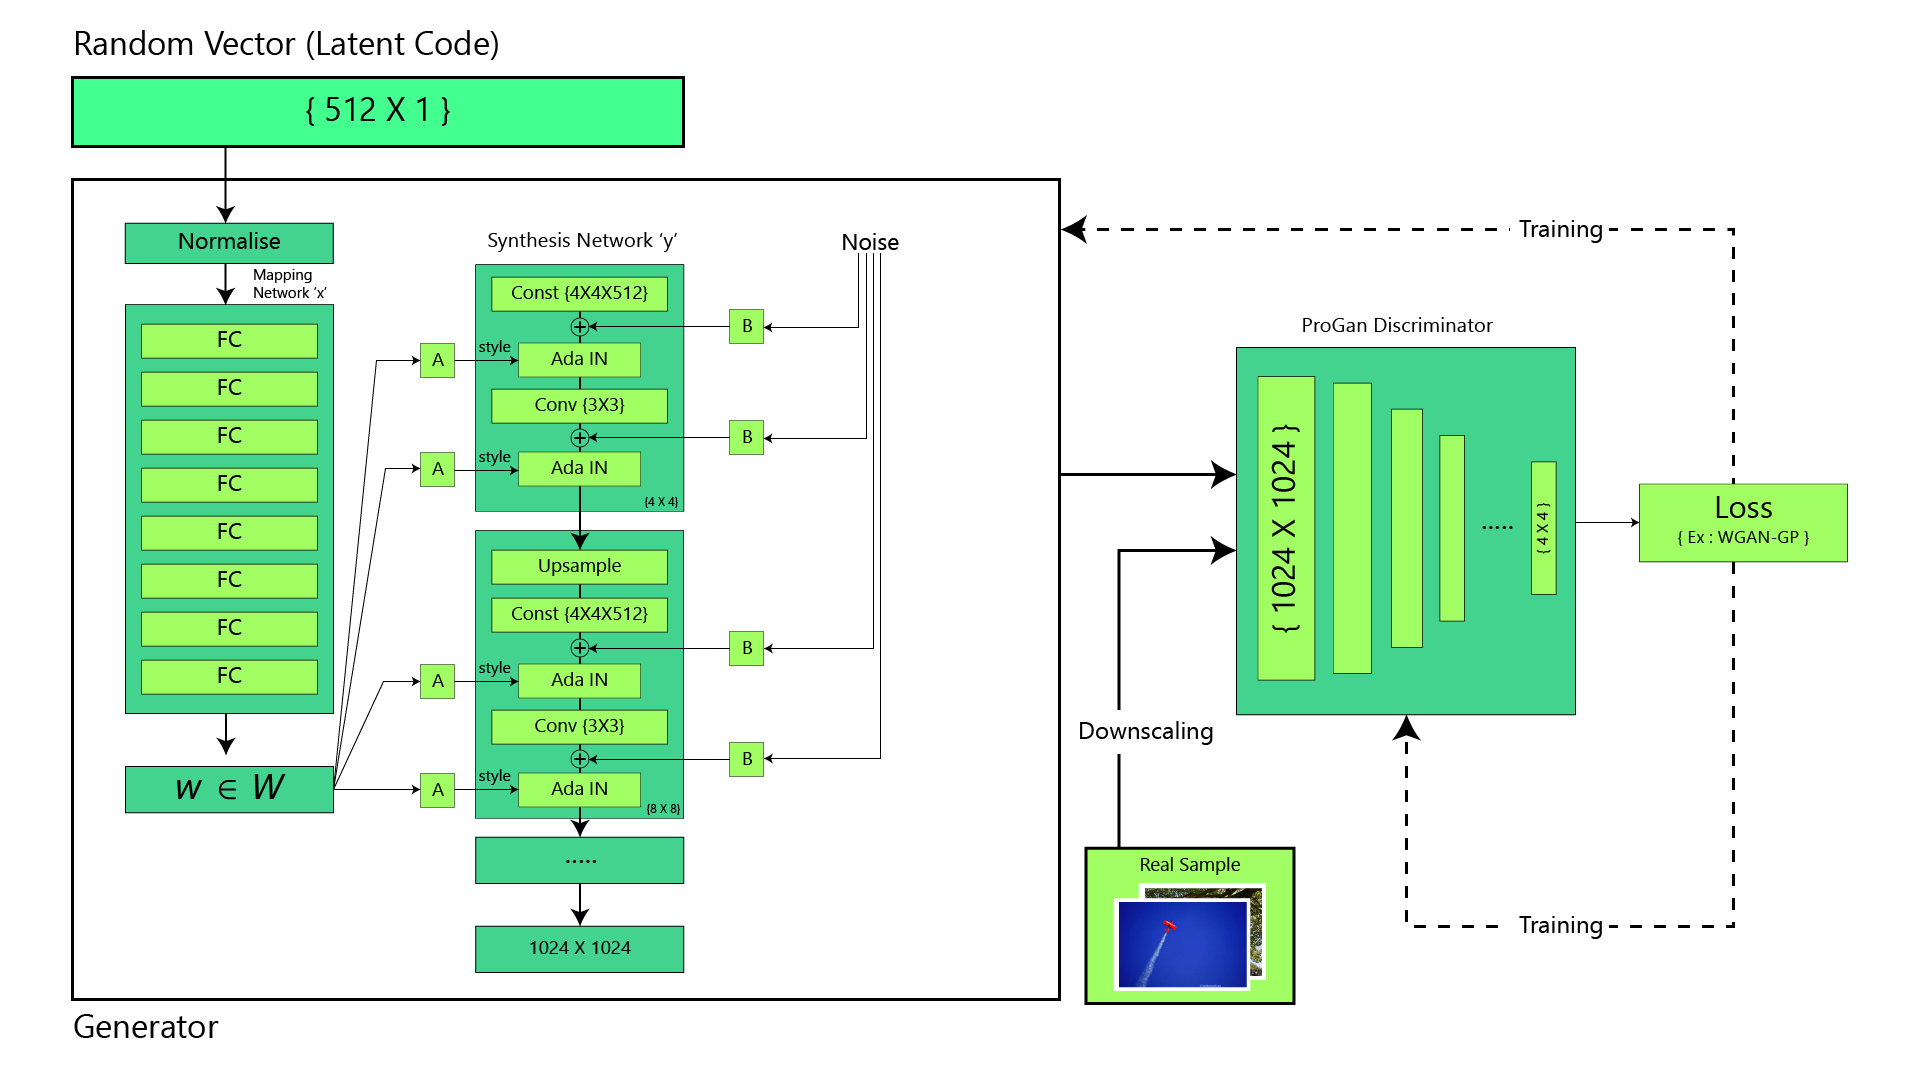
\includegraphics[width=1.0\textwidth]{images/stylegan_architecture.jpg}
	\captionof{figure}{Kiến trúc Generator dựa trên phong cách trong StyleGAN. Vector tiềm ẩn $\mathbf{z}$ được ánh xạ thành $\mathbf{w}$ qua Mapping Network, sau đó $\mathbf{w}$ điều khiển các lớp tích chập thông qua các module AdaIN để tạo ảnh với các đặc trưng ở nhiều cấp độ.}
	\label{fig:stylegan_architecture}
\end{center}

\subsection{Conditional GAN và CycleGAN: Sinh ảnh có Điều kiện}
\label{subsec:conditional_cyclegan}

\subsubsection{Conditional GAN (cGAN)}
\label{subsubsec:cgan}

GAN cơ bản sinh ảnh không kiểm soát được output. \textbf{Conditional GAN (cGAN)} \cite{Mirza2014} giải quyết vấn đề này bằng cách cung cấp một thông tin điều kiện $y$ cho cả Generator và Discriminator.

\textbf{Cơ chế hoạt động:}
\begin{itemize}
	\item \textbf{Generator ($G$):} Sinh ảnh giả $G(\mathbf{z}|y)$ dựa trên nhiễu $\mathbf{z}$ và điều kiện $y$ (ví dụ: nhãn lớp, ảnh khác, hoặc văn bản). Mục tiêu là tạo ra ảnh giả phù hợp với điều kiện, đánh lừa Discriminator.
	\item \textbf{Discriminator ($D$):} Phân biệt các cặp (ảnh, điều kiện) thật và giả. Như vậy, D không chỉ xem ảnh, mà còn xem điều kiện đi kèm để đưa ra quyết định.
\end{itemize}

\textbf{Ứng dụng:} cGAN mở ra khả năng sinh ảnh theo lớp cụ thể, chuyển đổi ảnh-sang-ảnh (image-to-image translation) như Pix2Pix, hoặc sinh ảnh dựa trên mô tả văn bản.  

\begin{center}
	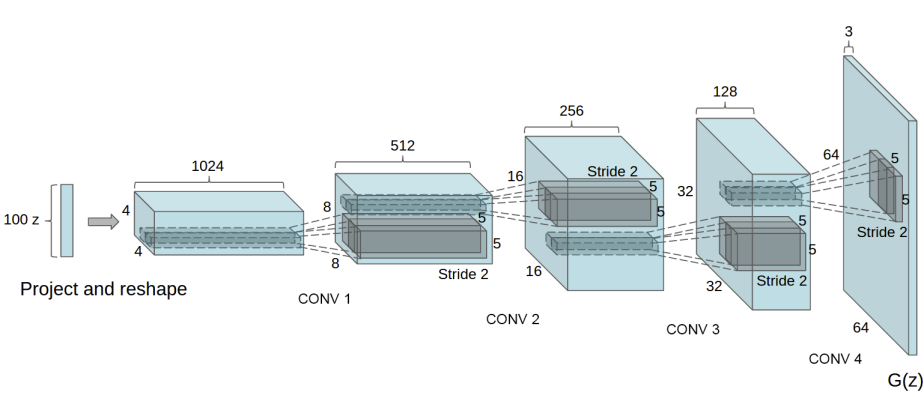
\includegraphics[width=0.9\textwidth]{images/cgan_architecture.png}
	\captionof{figure}{Cơ chế Conditional GAN: Generator sinh ảnh dựa trên điều kiện $y$, Discriminator phân biệt các cặp (ảnh, điều kiện) thật và giả.}
	\label{fig:cgan_architecture}
\end{center}

\subsubsection{CycleGAN (2017): Chuyển đổi Ảnh không cần Dữ liệu cặp}
\label{subsubsec:cyclegan}

Các mô hình như Pix2Pix yêu cầu các cặp ảnh (input, output) chính xác, điều này thường khó thực hiện. \textbf{CycleGAN} \cite{Zhu2017} cho phép chuyển đổi ảnh-sang-ảnh \textbf{không cần dữ liệu cặp (unpaired)} bằng cách huấn luyện đồng thời hai cặp Generator-Discriminator.

\textbf{Cơ chế hoạt động:}
\begin{itemize}
	\item \textbf{Generator $G: X \rightarrow Y$} học cách biến đổi ảnh từ miền X sang miền Y (ví dụ: ngựa $\rightarrow$ ngựa vằn).
	\item \textbf{Generator $F: Y \rightarrow X$} học cách chuyển ngược lại.
	\item \textbf{Discriminator $D_X$ và $D_Y$} phân biệt ảnh thật và ảnh giả trong từng miền.
	\item \textbf{Cycle-Consistency Loss:} Đảm bảo rằng ảnh chuyển X $\rightarrow$ Y $\rightarrow$ X vẫn giống ảnh gốc:
	\begin{equation}
		\mathcal{L}_{\text{cycle}} = \mathbb{E}_{\mathbf{x} \sim X} \big[\| F(G(\mathbf{x})) - \mathbf{x} \|_1 \big] 
		+ \mathbb{E}_{\mathbf{y} \sim Y} \big[\| G(F(\mathbf{y})) - \mathbf{y} \|_1 \big].
	\end{equation}
\end{itemize}

\textbf{Ý nghĩa:} Cycle-consistency giúp các Generator vừa tạo ra ảnh trông giống miền đích, vừa giữ cấu trúc nội dung của ảnh gốc. CycleGAN đã mở ra vô số ứng dụng sáng tạo, ví dụ: chuyển mùa, phong cách hội họa, hoặc chuyển ảnh thực sang ảnh nghệ thuật.

\begin{center}
	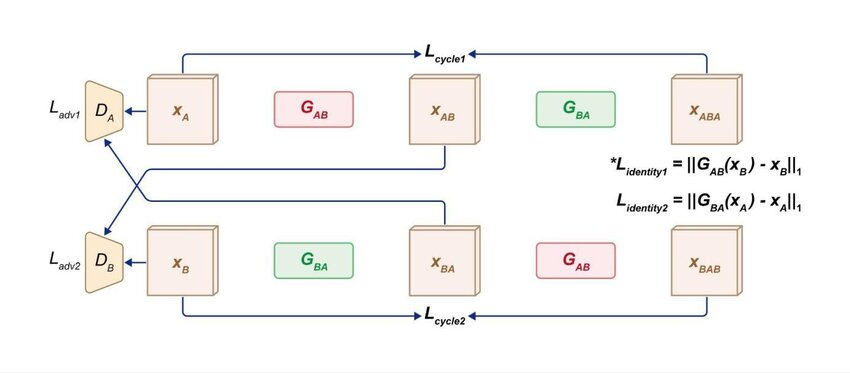
\includegraphics[width=1.0\textwidth]{images/cyclegan_architecture.png}
	\captionof{figure}{Kiến trúc CycleGAN: Hai Generator $G$ và $F$ học chuyển đổi hai chiều giữa miền X và Y, với các Discriminator tương ứng $D_X$ và $D_Y$. Cycle-consistency đảm bảo tính nhất quán của nội dung.}
	\label{fig:cyclegan_architecture}
\end{center}

\subsection{Các Phiên bản GAN Nổi bật Khác}
\label{subsec:advanced_gans}

Ngoài các GAN cơ bản, nhiều biến thể đã được phát triển để giải quyết các vấn đề về chất lượng ảnh, ổn định huấn luyện, điều khiển sinh ảnh, và chuyển đổi ảnh đa miền. Dưới đây là các phiên bản tiêu biểu:

\subsubsection{Progressive GAN (PGGAN, 2017)}
\textbf{Ý tưởng chính:} Huấn luyện GAN theo từng bước từ ảnh độ phân giải thấp lên cao.
\begin{itemize}
	\item \textbf{Cơ chế:} Bắt đầu sinh ảnh 4$\times$4, sau đó tăng dần lên 8$\times$8, 16$\times$16,... đến 1024$\times$1024. Mỗi bước thêm các layer mới vào Generator và Discriminator.
	\item \textbf{Ưu điểm:} Giúp GAN sinh ảnh độ phân giải cao, ổn định hơn, giảm khó khăn huấn luyện.
\end{itemize}

\subsubsection{Self-Attention GAN (SAGAN, 2018)}
\textbf{Ý tưởng chính:} Thêm cơ chế self-attention để Generator và Discriminator có khả năng quan sát toàn cảnh.
\begin{itemize}
	\item \textbf{Điểm mạnh:} Tăng chất lượng chi tiết và tính nhất quán của ảnh, đặc biệt với các đối tượng phức tạp hoặc cảnh quan.
\end{itemize}

\subsubsection{BigGAN (2018)}
\textbf{Ý tưởng chính:} Mở rộng GAN với quy mô lớn, batch size cực lớn và spectral normalization.
\begin{itemize}
	\item \textbf{Điểm mạnh:} Sinh ảnh chất lượng cao, chi tiết phong phú, đặc biệt hiệu quả với bộ dữ liệu ImageNet.
\end{itemize}

\subsubsection{Pix2PixHD (2018)}
\textbf{Ý tưởng chính:} Phiên bản nâng cấp của Pix2Pix, sinh ảnh cao phân giải cho tác vụ image-to-image translation.
\begin{itemize}
	\item \textbf{Cơ chế:} Kiến trúc multi-scale Generator và Discriminator, tăng độ sắc nét và chi tiết.
	\item \textbf{Ứng dụng:} Sketch $\rightarrow$ ảnh thực, bản đồ $\rightarrow$ ảnh vệ tinh, chuyển ảnh semantic $\rightarrow$ ảnh thực.
\end{itemize}

\subsubsection{StarGAN (2018)}
\textbf{Ý tưởng chính:} GAN đa miền (multi-domain) cho phép chuyển đổi ảnh sang nhiều miền khác nhau bằng một mô hình duy nhất.
\begin{itemize}
	\item \textbf{Ứng dụng:} Biểu cảm khuôn mặt, thay đổi tuổi, màu tóc, hoặc phong cách nghệ thuật.
\end{itemize}

\subsubsection{StyleGAN2-ADA (2020)}
\textbf{Ý tưởng chính:} Cải tiến StyleGAN2 kết hợp Adaptive Data Augmentation (ADA) để huấn luyện với dữ liệu nhỏ.
\begin{itemize}
	\item \textbf{Điểm mạnh:} Sinh ảnh ổn định, giảm artifact, chống overfitting trên tập dữ liệu hạn chế.
\end{itemize}

\subsubsection{MUNIT / DRIT (2018–2019)}
\textbf{Ý tưởng chính:} Image-to-image translation đa phong cách (multi-modal) bằng cách tách thông tin nội dung và phong cách.
\begin{itemize}
	\item \textbf{Cơ chế:} Mỗi ảnh input có thể được chuyển sang nhiều phong cách output khác nhau.
	\item \textbf{Ứng dụng:} Chuyển ảnh mùa hè $\leftrightarrow$ mùa đông, ảnh thực $\leftrightarrow$ tranh vẽ, phong cách anime hoặc nghệ thuật.
\end{itemize}

\textbf{Tóm tắt:} Các phiên bản GAN này đã mở rộng khả năng sinh ảnh, cải thiện độ ổn định huấn luyện và cung cấp khả năng kiểm soát quá trình sinh, từ ảnh cao phân giải, chi tiết phong phú, đến chuyển đổi đa miền và đa phong cách. Chúng tạo thành nền tảng cho nhiều ứng dụng sáng tạo trong thị giác máy tính và nghệ thuật số.

\subsection{Kết luận và Di sản}
\label{subsec:gan_conclusion_legacy}
GANs đã thống trị lĩnh vực mô hình sinh thị giác trong gần một thập kỷ. Chúng đã dạy cho cộng đồng nghiên cứu về tầm quan trọng của các hàm mất mát đối kháng, sự ổn định trong huấn luyện, và các kiến trúc cho phép điều khiển quá trình sinh. Các mô hình như \textbf{Progressive GAN}, \textbf{Self-Attention GAN (SAGAN)}, và \textbf{BigGAN} đã liên tục đẩy giới hạn về chất lượng và độ phân giải của ảnh sinh ra.

Mặc dù ngày nay, các mô hình khuếch tán (Diffusion Models) đã vượt qua GANs về chất lượng ảnh và sự đa dạng trong nhiều tác vụ, di sản của GANs vẫn còn đó. Các ý tưởng về không gian tiềm ẩn, các kiến trúc generator, và đặc biệt là tư duy đối kháng vẫn tiếp tục là nguồn cảm hứng và là một phần quan trọng trong bộ công cụ của các nhà nghiên cứu AI.

\section*{Tài liệu tham khảo}
\begin{itemize}
	\item[1] Goodfellow, I., Pouget-Abadie, J., Mirza, M., Xu, B., Warde-Farley, D., Ozair, S., ... \& Bengio, Y. (2014). Generative adversarial nets. In \textit{Advances in neural information processing systems (NeurIPS)}. (Paper gốc giới thiệu GAN).
	\item[2] Radford, A., Metz, L., \& Chintala, S. (2015). Unsupervised representation learning with deep convolutional generative adversarial networks. \textit{arXiv preprint arXiv:1511.06434}. (Paper gốc giới thiệu DCGAN).
	\item[3] Arjovsky, M., Chintala, S., \& Bottou, L. (2017). Wasserstein gan. \textit{arXiv preprint arXiv:1701.07875}. (Paper gốc giới thiệu WGAN).
	\item[4] Karras, T., Laine, S., \& Aila, T. (2019). A style-based generator architecture for generative adversarial networks. In \textit{Proceedings of the IEEE/CVF conference on computer vision and pattern recognition (CVPR)}. (Paper gốc giới thiệu StyleGAN).
	\item[5] Karras, T., Aittala, M., Laine, S., Härkönen, E., Hellsten, J., Lehtinen, J., \& Aila, T. (2021). Alias-free generative adversarial networks. In \textit{Advances in Neural Information Processing Systems (NeurIPS)}. (Paper giới thiệu StyleGAN3).
	\item[6] Mirza, M., \& Osindero, S. (2014). Conditional generative adversarial nets. \textit{arXiv preprint arXiv:1411.1784}. (Paper gốc giới thiệu cGAN).
	\item[7] Zhu, J. Y., Park, T., Isola, P., \& Efros, A. A. (2017). Unpaired image-to-image translation using cycle-consistent adversarial networks. In \textit{Proceedings of the IEEE international conference on computer vision (ICCV)}. (Paper gốc giới thiệu CycleGAN).
	\item[8] Brock, A., Donahue, J., \& Simonyan, K. (2018). Large scale gan training for high fidelity natural image synthesis. \textit{arXiv preprint arXiv:1809.11096}. (Paper giới thiệu BigGAN).
\end{itemize}